\documentclass[11pt,a4paper]{report}

% ---------------------------------------------------------------------------
% Packages
% ---------------------------------------------------------------------------
\usepackage[utf8]{inputenc}
\usepackage[T1]{fontenc}
\usepackage{textcomp}
\usepackage{geometry}
\geometry{margin=1in}
\usepackage{titlesec}
\usepackage{fancyhdr}
\usepackage{xcolor}
\usepackage{listings}
\usepackage{longtable}
\usepackage{booktabs}
\usepackage{array}
\usepackage{hyperref}
\usepackage{enumitem}
\usepackage{tikz}
\usetikzlibrary{arrows.meta, positioning, fit, backgrounds}
\usepackage{caption}
\usepackage{parskip}
\usepackage{amssymb}
\usepackage{tocloft}

% ---------------------------------------------------------------------------
% Colors
% ---------------------------------------------------------------------------
\definecolor{codebg}{RGB}{245,245,245}
\definecolor{codekeyword}{RGB}{0,0,150}
\definecolor{codecomment}{RGB}{100,100,100}
\definecolor{codestring}{RGB}{163,21,21}
\definecolor{headingblue}{RGB}{20,50,90}
\definecolor{tablehead}{RGB}{230,230,240}

% ---------------------------------------------------------------------------
% Code listings style
% ---------------------------------------------------------------------------
\lstdefinestyle{code}{
    backgroundcolor=\color{codebg},
    basicstyle=\ttfamily\small,
    keywordstyle=\color{codekeyword}\bfseries,
    commentstyle=\color{codecomment}\itshape,
    stringstyle=\color{codestring},
    breaklines=true,
    breakatwhitespace=false,
    showstringspaces=false,
    frame=single,
    rulecolor=\color{gray!40},
    numbers=left,
    numberstyle=\tiny\color{gray},
    numbersep=8pt,
    tabsize=4,
    xleftmargin=1em,
    framexleftmargin=1em,
    aboveskip=8pt,
    belowskip=8pt
}
\lstset{style=code}

\lstdefinelanguage{jsonlang}{
    basicstyle=\ttfamily\small,
    string=[s]{"}{"},
    stringstyle=\color{codestring},
    comment=[l]{//},
    commentstyle=\color{codecomment},
    morestring=[b]"
}

% ---------------------------------------------------------------------------
% Section formatting
% ---------------------------------------------------------------------------
\titleformat{\chapter}[display]
  {\normalfont\huge\bfseries\color{headingblue}}
  {\chaptertitlename\ \thechapter}{20pt}{\Huge}
\titleformat{\section}
  {\normalfont\Large\bfseries\color{headingblue}}
  {\thesection}{1em}{}
\titleformat{\subsection}
  {\normalfont\large\bfseries\color{headingblue}}
  {\thesubsection}{1em}{}

\pagestyle{fancy}
\fancyhf{}
\fancyhead[L]{\small\textit{FinSight Technical Documentation}}
\fancyhead[R]{\small\thepage}
\renewcommand{\headrulewidth}{0.4pt}

\hypersetup{
    colorlinks=true,
    linkcolor=headingblue,
    filecolor=magenta,
    urlcolor=blue,
    citecolor=headingblue,
    pdftitle={FinSight: Regulatory-Grade Financial Intelligence System -- Technical Documentation},
    pdfauthor={FinSight Engineering}
}

\newcommand{\code}[1]{\texttt{#1}}
\newcommand{\file}[1]{\texttt{\small #1}}

% ---------------------------------------------------------------------------
\title{
    \vspace{-2cm}
    {\Huge\bfseries FinSight}\\[0.3cm]
    {\Large Regulatory-Grade Financial Intelligence System}\\[0.2cm]
    {\large Technical System Documentation}
}
\author{Generated Technical Reference}
\date{\today}

\begin{document}

\maketitle
\thispagestyle{empty}

\begin{abstract}
\noindent
FinSight is a multi-agent Retrieval-Augmented Generation (RAG) system for analyzing
corporate financial filings (annual reports) with an explicit design mandate for
\emph{compliance-grade trustworthiness} rather than conversational convenience. Every
claim surfaced to the user is traceable to a verbatim source citation (document, page,
snippet); claims that cannot be verified against retrieved evidence are hard-blocked
before reaching the output, not merely flagged. The system decomposes a user query into
subtasks via a Planner agent, retrieves evidence through a hybrid dense/sparse
retrieval pipeline, extracts candidate claims via an Analyst agent, verifies each claim
against its source through an entailment-checking Auditor agent, performs deterministic
cross-document comparison through a Comparator agent, and finally synthesizes a
structured Markdown report through a Synthesizer agent. Every run produces a
machine-readable audit log capturing the full decision trail. This document provides an
exhaustive technical reference to the codebase: architecture, module-by-module
responsibilities, data models, API surface, configuration, testing and evaluation
methodology, and deployment topology.
\end{abstract}

\tableofcontents
\listoffigures
\listoftables

% =============================================================================
\chapter{Introduction and Project Purpose}
% =============================================================================

\section{Overview}

FinSight (version 1.0.0) analyzes public annual reports -- in the shipped corpus,
FY2024--FY2026 filings for three Indian IT services companies (Infosys, TCS, and
Wipro) -- and answers analyst-style natural language queries such as cross-company
margin comparisons, revenue-driver analysis, risk-disclosure extraction, and capital
expenditure guidance comparison.

The project is deliberately engineered against a written specification
(\file{FinSight\_Project\_Specification.pdf}, at the repository root) and is framed in
its own design records (\file{docs/DECISIONS.md}) as differentiated from a "standard
GenAI portfolio project": rather than a single LLM call over retrieved context, it
implements a six-stage agent pipeline with hard verification gates, deterministic
arithmetic where correctness matters, and full auditability.

\section{Design Mandate}

Four requirements recur throughout the documentation and the code itself, and they
motivate essentially every architectural decision described in this document:

\begin{enumerate}[leftmargin=1.5em]
    \item \textbf{Traceability.} Every factual claim in a synthesized report must carry
    a citation: source document, page number, and verbatim snippet.
    \item \textbf{Hard blocking, not soft flagging.} Claims that cannot be entailed by
    retrieved evidence are removed from the final report entirely -- they are not shown
    to the user with a caveat. This is enforced by the Auditor agent
    (Section~\ref{sec:auditor}).
    \item \textbf{Cross-document reasoning as a first-class capability.} Comparing
    figures across multiple filings (e.g., Infosys vs.\ TCS, FY2024 vs.\ FY2025) is
    handled by a dedicated Comparator agent that performs \emph{no} LLM arithmetic --
    all currency/unit conversion is done deterministically in Python
    (Section~\ref{sec:unit-normalizer}) before the LLM ever compares figures.
    \item \textbf{Full auditability.} Every query execution persists a structured JSON
    audit log (Section~\ref{sec:auditlog}) recording the plan, every retrieval, every
    claim (verified, uncertain, or blocked), and every agent invoked, with end-to-end
    latency.
\end{enumerate}

\section{Confidence Model}

Rather than a binary answerable/unanswerable decision, FinSight assigns each claim a
composite confidence score (Section~\ref{sec:confidence}) and classifies it into one of
three tiers:

\begin{center}
\begin{tabular}{@{}lll@{}}
\toprule
\textbf{Status} & \textbf{Meaning} & \textbf{Surfaced to user?} \\
\midrule
\texttt{VERIFIED} & Entailed by evidence, confidence $\geq$ threshold & Yes \\
\texttt{UNCERTAIN} & Weak support or below threshold & Yes, prefixed \texttt{[UNCERTAIN]} \\
\texttt{UNVERIFIABLE} & Absent, contradictory, or fabricated-event pattern & No (blocked) \\
\bottomrule
\end{tabular}
\end{center}

% =============================================================================
\chapter{System Architecture}
% =============================================================================

\section{Orchestration Framework}

FinSight is orchestrated by Microsoft \textbf{Semantic Kernel} (SK), which the design
records describe as "load-bearing" infrastructure rather than a thin wrapper around
direct LLM calls. A single process-wide \code{Kernel} singleton is constructed by
\file{core/sk\_kernel.py}\code{::get\_kernel()} and registers:

\begin{itemize}
    \item One chat completion service (\code{OpenAIChatCompletion}), pointed at Groq's
    OpenAI-compatible endpoint (or an operator-configured fallback endpoint).
    \item Four \textbf{native plugins} -- Python classes decorated with
    \code{@kernel\_function} -- for agents that perform real deterministic or
    LLM-hybrid computation: \code{RetrieverPlugin}, \code{AnalystPlugin},
    \code{AuditorPlugin}, \code{ComparatorPlugin}.
    \item Two \textbf{semantic functions} (\code{KernelFunctionFromPrompt}, pure prompt
    templates rendered by the kernel) for agents that are pure text-in/text-out LLM
    tasks: \code{Planner.decompose} and \code{Synthesizer.synthesize}.
\end{itemize}

In practice, the Planner and Synthesizer prompt templates (\code{PLANNER\_PROMPT},
\code{SYNTHESIZER\_PROMPT} in \file{core/sk\_kernel.py}) are reused as raw format
strings and invoked via direct \code{chat\_completion()} /
\code{chat\_completion\_hedged()} calls in the API route handlers, rather than through
\code{kernel.invoke()}. Only the Retriever, Analyst, Auditor, and Comparator agents are
invoked through \code{kernel.invoke(plugin\_name=..., function\_name=...,
arguments=KernelArguments(...))}. This mixed design -- two different invocation
patterns for what is conceptually one pipeline -- is an explicit, documented tradeoff
in \file{docs/DECISIONS.md}.

\section{The Six-Stage Pipeline}
\label{sec:pipeline}

\begin{figure}[h]
\centering
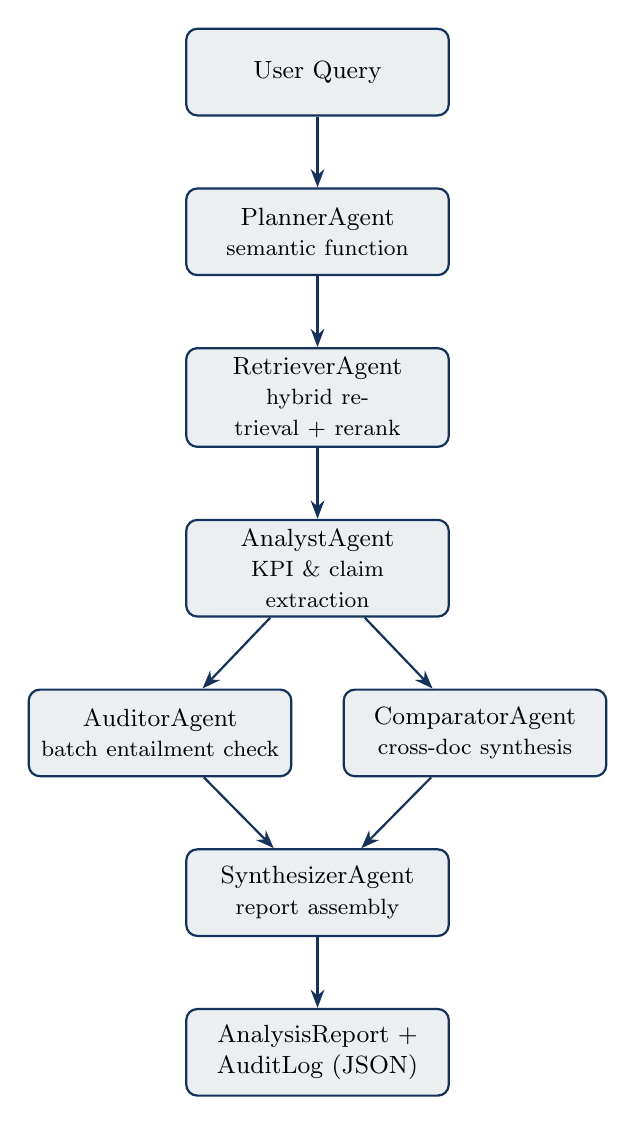
\begin{tikzpicture}[
    node distance=0.9cm and 1.6cm,
    box/.style={rectangle, draw=headingblue, thick, rounded corners, fill=headingblue!8,
                text width=3.1cm, align=center, minimum height=1.1cm, font=\small},
    arrow/.style={-Stealth, thick, headingblue}
]
\node[box] (query) {User Query};
\node[box, below=of query] (planner) {PlannerAgent\\\footnotesize semantic function};
\node[box, below=of planner] (retriever) {RetrieverAgent\\\footnotesize hybrid retrieval + rerank};
\node[box, below=of retriever] (analyst) {AnalystAgent\\\footnotesize KPI \& claim extraction};
\node[box, below=of analyst, xshift=-2.0cm] (auditor) {AuditorAgent\\\footnotesize batch entailment check};
\node[box, below=of analyst, xshift=2.0cm] (comparator) {ComparatorAgent\\\footnotesize cross-doc synthesis};
\node[box, below=of auditor, xshift=2.0cm] (synth) {SynthesizerAgent\\\footnotesize report assembly};
\node[box, below=of synth] (out) {AnalysisReport +\\AuditLog (JSON)};

\draw[arrow] (query) -- (planner);
\draw[arrow] (planner) -- (retriever);
\draw[arrow] (retriever) -- (analyst);
\draw[arrow] (analyst) -- (auditor);
\draw[arrow] (analyst) -- (comparator);
\draw[arrow] (auditor) -- (synth);
\draw[arrow] (comparator) -- (synth);
\draw[arrow] (synth) -- (out);
\end{tikzpicture}
\caption{The six-stage agent pipeline. Auditor and Comparator run concurrently in the
streaming route since neither depends on the other's output -- only on the shared
\code{subtask\_results}.}
\label{fig:pipeline}
\end{figure}

\begin{enumerate}[leftmargin=1.5em]
    \item \textbf{PlannerAgent} decomposes the user query into 2--6 subtasks (a JSON
    list of strings).
    \item \textbf{RetrieverAgent} (run per subtask, in parallel): hybrid BM25 + dense
    retrieval, Reciprocal Rank Fusion, cross-encoder reranking, and confidence scoring,
    producing ranked chunks with citations.
    \item \textbf{AnalystAgent} (per subtask): extracts KPIs and verbatim claims from
    the retrieved chunks via an LLM call constrained to forbid any derived/computed
    figure.
    \item \textbf{AuditorAgent}: a single batched LLM call verifies every claim
    produced by every subtask via entailment checking against its supporting snippet,
    classifying each as VERIFIED, UNCERTAIN, or UNVERIFIABLE.
    \item \textbf{ComparatorAgent} (runs concurrently with the Auditor): performs
    cross-document comparison of pre-normalized figures, flagging deltas exceeding a
    15\% deviation threshold, without performing any arithmetic itself.
    \item \textbf{SynthesizerAgent}: assembles a structured Markdown report from
    verified and uncertain claims plus the comparison output.
\end{enumerate}

\section{Context Propagation}

Citations and claims are threaded through the pipeline as JSON strings inside
\code{KernelArguments}, so no information is silently dropped between stages:

\begin{center}
\ttfamily\small
user\_task $\rightarrow$ subtasks (list[str]) $\rightarrow$ chunks\_json $\rightarrow$
analysis\_json (claims) $\rightarrow$ claims\_json $\rightarrow$ audit\_json
$\rightarrow$ comparison\_json $\rightarrow$ final report
\end{center}

\section{Concurrency and Latency Management}

The streaming route (\file{api/routes/query\_stream.py}) applies several
latency-reduction strategies:

\begin{itemize}
    \item All subtasks' Retriever + Analyst calls run in parallel via
    \code{asyncio.gather}.
    \item Auditor and Comparator run concurrently rather than sequentially, since
    neither consumes the other's output.
    \item \code{core/groq\_client.py}\code{::chat\_completion\_hedged()} implements
    \emph{request hedging}: the primary LLM call is fired first; if it has not
    returned within a configurable \code{hedge\_after} interval (8.0\,s in the
    streaming route), the reserve endpoint is fired concurrently and whichever
    completes first is used. This bounds tail (p95) latency without doubling average
    cost.
\end{itemize}

% =============================================================================
\chapter{Repository Layout}
% =============================================================================

\begin{lstlisting}[language=bash, basicstyle=\ttfamily\footnotesize, frame=single]
FinSight/
|-- agents/                    Six-stage agent pipeline (SK-orchestrated)
|   |-- router.py               PlannerAgent
|   |-- retriever.py            RetrieverPlugin (SK native plugin)
|   |-- analyst.py              AnalystPlugin (SK native plugin)
|   |-- comparator.py           ComparatorPlugin (SK native plugin)
|   |-- auditor.py              AuditorPlugin (SK native plugin)
|   `-- synthesizer.py          synthesize_report() (direct LLM call)
|-- api/                        FastAPI application
|   |-- main.py                 App factory, lifespan, static mounting, /health
|   |-- metrics_store.py        In-process MetricsStore singleton
|   |-- middleware/guardrails.py  Prompt-injection detection (pure ASGI)
|   |-- routes/
|   |   |-- query.py             POST /query (blocking pipeline)
|   |   |-- query_stream.py      POST /query/stream (SSE pipeline)
|   |   |-- ingest.py            POST /ingest/upload
|   |   |-- eval.py              GET /eval/*
|   |   `-- metrics.py           GET /metrics/json
|   `-- static/
|       |-- index.html           Web UI (query interface + pipeline visualizer)
|       `-- dashboard.html       Metrics dashboard
|-- core/                       Shared infrastructure
|   |-- config.py                pydantic-settings Settings (env vars)
|   |-- models.py                Dataclasses & enums
|   |-- sk_kernel.py             SK Kernel builder, prompt templates
|   |-- groq_client.py           Async LLM client: retry, fallback, hedging
|   `-- unit_normalizer.py       Deterministic INR/USD normalizer
|-- retrieval/                  Hybrid retrieval pipeline
|   |-- qdrant_store.py          Async Qdrant client wrapper
|   |-- embedder.py              SentenceTransformer wrapper
|   |-- bm25.py                  BM25Okapi wrapper
|   |-- hybrid.py                Reciprocal Rank Fusion
|   |-- reranker.py              CrossEncoder wrapper
|   `-- confidence.py            5-signal composite confidence scoring
|-- ingestion/                  PDF -> Qdrant ingestion pipeline
|   |-- parser.py                PyMuPDF page/block/span extraction
|   |-- chunker.py               Heading-aware sliding-window chunker
|   |-- metadata.py              Section/fiscal-year/company detection
|   `-- pipeline.py              ingest_pdf(), ingest_directory()
|-- observability/tracer.py     structlog config, @traced decorator, OTel setup
|-- evaluation/
|   |-- harness.py               Async CLI test runner
|   |-- queries/                 happy_path.json, adversarial.json
|   `-- results/                 Timestamped harness_<epoch>.json results
|-- tests/                      pytest unit tests
|-- scripts/download_filings.py Multi-strategy annual-report downloader
|-- data/filings/                Seed PDFs (Infosys / TCS / Wipro)
|-- audit_logs/                  Per-run JSON audit artifacts
|-- qdrant_storage/               Qdrant on-disk vector data
|-- docs/
|   |-- ARCHITECTURE.md          Architecture reference
|   `-- DECISIONS.md             Design-decision records
|-- .github/workflows/ci.yml     GitHub Actions CI (ruff + pytest)
|-- Dockerfile                    Multi-stage build
|-- docker-compose.yml            qdrant + api services
`-- pyproject.toml                Dependencies, ruff & pytest config
\end{lstlisting}

Two files, \file{retrieval/chunker.py} and \file{retrieval/dummy\_test.py}, are
development-era scratch duplicates of the canonical ingestion logic used for manual
PDF experimentation; they are not part of the production import graph reached by
\file{ingestion/pipeline.py}.

% =============================================================================
\chapter{Technology Stack}
% =============================================================================

\section{Core Dependencies}

Python $\geq$3.11, managed with \code{uv}. Key libraries declared in
\file{pyproject.toml}:

\begin{longtable}{@{}p{4cm}p{4cm}p{6.5cm}@{}}
\toprule
\textbf{Category} & \textbf{Library} & \textbf{Role} \\
\midrule
\endhead
PDF parsing & \code{pymupdf} (fitz) & Page/block/span text extraction \\
Vector database client & \code{qdrant-client} & Async Qdrant driver \\
Embeddings \& reranking & \code{sentence-transformers} & Bi-encoder and cross-encoder models \\
Keyword search & \code{rank-bm25} & BM25Okapi sparse retrieval \\
Orchestration & \code{semantic-kernel} & Agent/plugin orchestration \\
LLM client & \code{openai} & OpenAI-compatible client pointed at Groq \\
LLM client (alt.) & \code{groq} & Native Groq SDK \\
API framework & \code{fastapi} & HTTP API \\
ASGI server & \code{uvicorn[standard]} & Application server \\
Configuration & \code{pydantic-settings} & Typed env-var settings \\
Logging & \code{structlog} & Structured logging \\
HTTP client & \code{httpx} & Async HTTP \\
Numerics & \code{numpy} & Vector math \\
Observability & \code{opentelemetry-*} & Tracing (OTLP/gRPC exporter) \\
Uploads & \code{python-multipart} & Multipart form parsing \\
\bottomrule
\end{longtable}

Development dependencies: \code{pre-commit}, \code{ruff} (line-length 100, target
py311, rule sets E/F/I), \code{pytest} + \code{pytest-asyncio}
(\code{asyncio\_mode="auto"}), \code{httpx} (for test client usage).

\section{External Services}

\begin{itemize}
    \item \textbf{Qdrant} -- vector database, collection \code{finsight\_chunks},
    384-dimensional vectors (matching \code{all-MiniLM-L6-v2}), cosine distance.
    \item \textbf{Groq} -- hosts the primary LLM, \textbf{Llama 3.3 70B}
    (\code{llama-3.3-70b-versatile}), via an OpenAI-compatible API. An optional reserve
    endpoint (any OpenAI-compatible provider) can be configured for hedging/failover.
\end{itemize}

\section{Frontend}

The UI (\file{api/static/index.html}, \file{dashboard.html}) is plain HTML/CSS/JS --
no JavaScript framework -- styled as a dark "compliance terminal" with a live pipeline
visualizer that consumes the \code{/query/stream} SSE events, plus a separate metrics
dashboard consuming \code{/metrics/json}.

% =============================================================================
\chapter{Module Reference}
% =============================================================================

This chapter documents every module's responsibility, key functions, and
inputs/outputs.

\section{Agents (\file{agents/})}

\subsection{\file{router.py} --- PlannerAgent}

\begin{lstlisting}[language=Python]
def plan_task(user_task: str) -> list[str]:
    ...
\end{lstlisting}

Invokes \code{kernel.invoke(plugin\_name="Planner", function\_name="decompose",
arguments=KernelArguments(user\_task=...))}. Parses the LLM's JSON list output; on
JSON-parse failure falls back to bullet/numbered-list regex parsing; if that also fails,
falls back to the single-element list \code{[user\_task]}.

\subsection{\file{retriever.py} --- RetrieverPlugin}
\label{sec:retriever}

\code{RetrieverPlugin} exposes a single \code{@kernel\_function(name="retrieve")}
method:

\begin{lstlisting}[language=Python]
def retrieve(subtask, company_filter="", fiscal_year_filter="") -> str:  # JSON
\end{lstlisting}

It lazily builds a BM25 index once per process (guarded by an \code{asyncio.Lock} with
double-checked initialization) over the full Qdrant corpus, obtained via
\code{scroll\_all()}. The real work is delegated to the module-level
\code{retrieve\_chunks()}, which:

\begin{enumerate}
    \item Filters BM25 payloads in-memory for company/fiscal-year (handling
    \code{"FY2024"} vs.\ \code{"2024"} via substring matching, since Qdrant's exact-match
    filter cannot).
    \item Embeds the query.
    \item Runs BM25 search and dense Qdrant search concurrently
    (\code{asyncio.gather}).
    \item Fuses the two ranked lists via Reciprocal Rank Fusion.
    \item Reranks the fused candidates via a cross-encoder.
    \item Builds \code{RankedChunk} objects with composite confidence scores.
\end{enumerate}

\subsection{\file{analyst.py} --- AnalystPlugin}

\begin{lstlisting}[language=Python]
def analyze(subtask, chunks_json) -> str:  # JSON {"kpis": [...], "claims": [...]}
\end{lstlisting}

Delegates to \code{analyze\_chunks()}, which builds a context string from up to
\code{settings.rerank\_top\_k} chunks and calls the LLM with a strict system prompt
that \textbf{forbids extracting any derived or computed figure} -- ratios, per-unit
metrics, currency conversions, or cross-company combinations are disallowed; only
verbatim printed figures may become claims. Confidence is assigned deterministically by
section type (0.9 audited financials / 0.75 notes / 0.6 MD\&A-or-letter). At most five
claims are extracted per call. On JSON-parse failure, a regex-based fallback extraction
is applied.

\subsection{\file{auditor.py} --- AuditorPlugin}
\label{sec:auditor}

\begin{lstlisting}[language=Python]
def audit(claims_json, confidence_threshold="0.65", original_query="") -> str:
\end{lstlisting}

Core logic lives in \code{audit\_claims()}. Claims are split into two groups:

\begin{itemize}
    \item Claims \emph{with} a supporting snippet: batch-audited in a \textbf{single}
    LLM call (\code{\_batch\_entailment()}) for efficiency and consistency.
    \item Claims \emph{without} a supporting snippet: instantly classified
    \code{UNVERIFIABLE} with reason \code{"No supporting snippet provided"} -- no LLM
    call needed.
\end{itemize}

The batch-entailment prompt applies two checks, in order:

\begin{enumerate}
    \item \textbf{Fabricated-event detection}: if the original query names a specific
    external company plus an action verb, and the claim's topic is unrelated, the
    claim is forced to \code{UNVERIFIABLE} regardless of superficial snippet overlap.
    This targets adversarial queries such as "what did the CEO say about acquiring
    Google."
    \item \textbf{Standard entailment classification}: \code{VERIFIED} if the snippet
    entails the claim and confidence $\geq$ threshold; \code{UNCERTAIN} if support is
    weak or confidence is below threshold; \code{UNVERIFIABLE} if the snippet is
    absent or contradicts the claim.
\end{enumerate}

Returns a triple \code{(verified, uncertain, unverifiable)} of \code{AuditedClaim}
lists.

\subsection{\file{comparator.py} --- ComparatorPlugin}

\begin{lstlisting}[language=Python]
def compare(subtask_results_json, original_query) -> str:
\end{lstlisting}

Delegates to \code{compare\_results()}, which calls the LLM under a system prompt that
\textbf{prohibits any arithmetic}: no per-unit metrics, no currency/scale conversion, no
percentage-delta computation, no cross-company arithmetic. The LLM's sole job is to
place pre-normalized (already converted to Rs.\ crore) verbatim
values side by side and flag anomalies -- deviations exceeding 15\% between comparable
figures, unit/currency mismatches, or contradictions with auditor statements. Output:
\begin{lstlisting}[language=jsonlang]
{"deltas": [...], "cross_document_claims": [...], "summary": "..."}
\end{lstlisting}

\subsection{\file{synthesizer.py} --- SynthesizerAgent}

\begin{lstlisting}[language=Python]
def synthesize_report(query, verified_claims, uncertain_claims,
                       comparison, task_id) -> str:
\end{lstlisting}

A direct \code{chat\_completion()} call (not SK tool-calling) using the
\code{SYNTHESIZER\_PROMPT} template from \file{core/sk\_kernel.py}. Returns an
"insufficient evidence" message outright if there are no verified or uncertain claims.
The prompt enforces: only verbatim figures with inline citations; an
\code{[UNCERTAIN]} prefix on uncertain claims; omission of derived figures unless
pre-labeled \code{[converted from ...]}; no arithmetic; explicit \code{N/A} for missing
data; and a fixed GitHub-Flavored-Markdown section structure (Executive Summary / Key
Findings / Comparative Analysis / Risk Flags).

\section{Core Infrastructure (\file{core/})}

\subsection{\file{config.py}}

\code{Settings(BaseSettings)} -- a \code{pydantic-settings} model reading \file{.env}.
All fields are enumerated in Table~\ref{tab:config}.

\subsection{\file{models.py}}

The canonical dataclasses and enums shared across the entire system; see
Chapter~\ref{ch:models}.

\subsection{\file{sk\_kernel.py}}

Builds and holds the SK \code{Kernel} singleton (\code{get\_kernel()}), an optional
reserve kernel (\code{get\_fallback\_kernel()}), and \code{reset\_kernel()}. Contains the
\code{PLANNER\_PROMPT} and \code{SYNTHESIZER\_PROMPT} string templates and registers
native plugins plus semantic functions inside \code{\_build\_kernel()}.

\subsection{\file{groq\_client.py}}

Lazily-initialized singleton \code{AsyncOpenAI} clients (primary, and optionally a
reserve client selected when fallback environment variables are set).

\begin{itemize}
    \item \code{chat\_completion()}: retries on \code{RateLimitError} / HTTP 503 with
    backoff \code{[1.0, 2.0, 4.0]} seconds; breaks immediately to the reserve client on
    timeout or connection errors; raises \code{RuntimeError} if both primary and
    reserve fail.
    \item \code{chat\_completion\_hedged()}: implements the hedged dual-request pattern
    described in Section~\ref{sec:pipeline} -- fires the primary request, and after a
    configurable delay fires the reserve concurrently, returning whichever completes
    first.
\end{itemize}

\subsection{\file{unit\_normalizer.py}}
\label{sec:unit-normalizer}

A pure-Python, regex-driven, deterministic currency/unit normalizer:
\code{normalize\_text()} and \code{normalize\_subtask\_results()}. Converts expressions
such as \code{\$X billion/million/...} and \code{Rs/INR X
crore/lakh/million/...} into a canonical \code{Rs. X crore [converted from
...]} form using \code{Decimal} arithmetic (\code{USD\_TO\_INR = 84}). This module
exists specifically so that the Comparator and Synthesizer LLM stages never perform
currency or scale arithmetic themselves -- all such conversion happens deterministically
in Python before the LLM sees the data, eliminating a whole class of hallucinated
arithmetic.

\section{Retrieval Pipeline (\file{retrieval/})}

\begin{description}
    \item[\file{qdrant\_store.py}] \code{QdrantStore} wraps \code{AsyncQdrantClient}:
    \code{ensure\_collection()} (384-dim, cosine distance), \code{upsert\_chunks()},
    \code{dense\_search()} (with optional payload \code{Filter}), \code{scroll\_all()}
    (paginated full-corpus fetch feeding the BM25 index), \code{delete\_by\_doc\_id()},
    \code{collection\_info()}.
    \item[\file{embedder.py}] Lazy \code{SentenceTransformer(all-MiniLM-L6-v2)}
    singleton; \code{embed\_query()}, \code{embed\_texts()} (normalized embeddings).
    \item[\file{bm25.py}] \code{BM25Retriever} wraps \code{rank\_bm25.BM25Okapi}; a
    custom \code{\_tokenize()} regex deliberately keeps \code{\%} attached to its
    number (so \code{20.7\%} tokenizes as one token) since financial figures with
    percent signs are common retrieval targets.
    \item[\file{hybrid.py}] \code{reciprocal\_rank\_fusion(ranked\_lists, k=60)} -- a
    purely rank-based fusion that is invariant to the differing score scales of BM25
    and cosine similarity.
    \item[\file{reranker.py}] Lazy \code{CrossEncoder(ms-marco-MiniLM-L6-v2)}
    singleton; \code{rerank(query, candidates, top\_k)} replaces stage-1 fused scores
    entirely with cross-encoder relevance scores.
    \item[\file{confidence.py}] \code{compute\_confidence()} and
    \code{build\_ranked\_chunks()}; see Section~\ref{sec:confidence}.
\end{description}

\subsection{Confidence Scoring}
\label{sec:confidence}

\code{compute\_confidence()} computes a weighted composite of five signals:

\begin{center}
\begin{tabular}{@{}lcl@{}}
\toprule
\textbf{Signal} & \textbf{Weight} & \textbf{Description} \\
\midrule
Retrieval score & 35\% & Cross-encoder rerank score \\
Section-type weight & 25\% & Static weight by document section (see Table~\ref{tab:section-weights}) \\
Freshness & 15\% & Decays 0.2/year from a 2025 baseline, floor 0.2 \\
Cross-filing consistency & 15\% & 1.0 if $\geq$3 same-company docs corroborate, 0.75 if 2, else 0.4 \\
Retrieval consistency & 10\% & Computed from \code{query\_variants\_hit} (placeholder signal) \\
\bottomrule
\end{tabular}
\end{center}

\section{Ingestion Pipeline (\file{ingestion/})}

\begin{description}
    \item[\file{parser.py}] \code{parse\_pdf()} (page/block dictionaries),
    \code{extract\_text\_with\_positions()} (span-level with bounding boxes),
    \code{get\_page\_text()} -- all via PyMuPDF.
    \item[\file{chunker.py}] \code{chunk\_document(pages, doc\_id, source,
    target\_tokens=400, overlap\_tokens=80)}: a heading-aware sliding window. Headings
    are detected via a font-size heuristic (\code{span.size > body\_size * 1.2}); a new
    chunk starts at a heading boundary once enough tokens have accumulated, otherwise
    the window slides with overlap. \code{chunk\_id} is a SHA-256 hash of
    \code{(doc\_id, page, index, text[:100])}. \code{\_deduplicate()} drops chunks
    whose first 200 characters hash identically, keeping the first occurrence.
    \item[\file{metadata.py}] \code{detect\_section\_type()} (regex cascade: audited
    financials $\to$ notes $\to$ MD\&A $\to$ letter $\to$ unknown, with a
    \code{"note"} sub-check redirecting some audited-financials matches to NOTES),
    \code{detect\_fiscal\_year()} (regex \code{FY\textbackslash d\{4\}}, falling back
    to a bare-year scan 2024 $\to$ 2020), \code{detect\_company()} (filename plus
    first-200-character text hints for Infosys/TCS/Wipro, handling
    underscore/hyphen normalization and a "Tata Consultancy" alias),
    \code{section\_type\_confidence\_weight()} (weights 1.0 / 0.85 / 0.65 / 0.40 / 0.50
    -- see note in Table~\ref{tab:section-weights}).
    \item[\file{pipeline.py}] \code{ingest\_pdf(pdf\_path, doc\_id=None,
    overwrite=True)}: parse $\to$ chunk $\to$ batch-embed $\to$
    \code{ensure\_collection()} $\to$ optional \code{delete\_by\_doc\_id()} (for
    re-ingestion idempotency) $\to$ \code{upsert\_chunks()}.
    \code{ingest\_directory(directory, pattern="*.pdf")}: batch-ingests every matching
    file, capturing per-file errors without aborting the batch.
\end{description}

\begin{table}[h]
\centering
\caption{Section-type confidence weights as implemented in code (authoritative)
versus as documented in \file{docs/ARCHITECTURE.md}. The code values govern actual
system behavior.}
\label{tab:section-weights}
\begin{tabular}{@{}lcc@{}}
\toprule
\textbf{Section type} & \textbf{Code weight} & \textbf{Docs-stated weight} \\
\midrule
Audited financials & 1.00 & 1.0 \\
Notes & 0.85 & 0.8 \\
MD\&A & 0.65 & 0.7 \\
Letter & 0.40 & 0.5 \\
Unknown & 0.50 & 0.4 \\
\bottomrule
\end{tabular}
\end{table}

\section{Observability (\file{observability/tracer.py})}

\code{setup\_tracing()} is idempotent (guarded by a \code{\_configured} flag) and
configures \code{structlog} with either a \code{ConsoleRenderer} (text format) or
\code{JSONRenderer} (JSON / OpenTelemetry-enabled format), merging context variables and
adding log level plus ISO timestamp. When \code{OTEL\_ENABLED} is set, an OpenTelemetry
\code{TracerProvider} with an \code{OTLPSpanExporter} is additionally configured. The
\code{traced(name=None)} decorator logs start/complete/error events with millisecond
latency for any decorated async function.

% =============================================================================
\chapter{Data Models}
\label{ch:models}
% =============================================================================

All models are defined in \file{core/models.py} as \code{dataclasses}
(\code{from \_\_future\_\_ import annotations}).

\section{Enumerations}

\begin{lstlisting}[language=Python]
class SectionType(str, Enum):
    AUDITED_FINANCIALS = "audited_financials"
    MDA = "mda"
    NOTES = "notes"
    LETTER = "letter"
    UNKNOWN = "unknown"

class AuditStatus(str, Enum):
    VERIFIED = "verified"
    UNCERTAIN = "uncertain"
    UNVERIFIABLE = "unverifiable"
\end{lstlisting}

\section{Core Dataclasses}

\begin{lstlisting}[language=Python]
@dataclass
class Citation:
    document: str
    page: int
    snippet: str
    claim: str
    confidence: float
    section_type: str
    # to_dict()

@dataclass
class Chunk:
    chunk_id: str
    doc_id: str
    source: str
    text: str
    page: int
    section: str
    section_type: SectionType
    token_count: int
    fiscal_year: str = ""
    company: str = ""
    # to_payload() / from_payload() -- Qdrant payload (de)serialization

@dataclass
class RankedChunk:
    chunk: Chunk
    retrieval_score: float
    confidence_score: float
    # to_citation(claim="") -> Citation

@dataclass
class AuditedClaim:
    claim: str
    citation: Citation
    audit_status: AuditStatus
    audit_reason: str
    # to_dict()

@dataclass
class SubtaskResult:
    subtask: str
    ranked_chunks: list[RankedChunk]
    kpis: list[dict]
    claims: list[AuditedClaim]
    agents_used: list[str] = field(default_factory=list)

@dataclass
class AuditLog:
    task_id: str
    timestamp: str
    user_query: str
    plan: list[str]
    retrievals: dict[str, list[str]]
    claims: list[dict]
    flagged_uncertain: list[str]
    blocked_unverifiable: list[str]
    agents_invoked: list[str]
    latency_ms: int
    # to_dict()

@dataclass
class AnalysisReport:
    task_id: str
    query: str
    summary: str
    verified_claims: list[AuditedClaim]
    uncertain_claims: list[AuditedClaim]
    audit_log: AuditLog
    # to_dict()
\end{lstlisting}

\section{Qdrant Collection Schema}

Collection \code{finsight\_chunks}: 384-dimensional vectors
(\code{all-MiniLM-L6-v2}), cosine distance. Payload fields: \code{chunk\_id},
\code{doc\_id}, \code{source}, \code{text}, \code{page}, \code{section},
\code{section\_type}, \code{token\_count}, \code{fiscal\_year}, \code{company}.
Payload-level filtering is used for \code{company} during dense search directly in
Qdrant; fiscal-year filtering is instead performed in-memory over the BM25 payload set,
since Qdrant's filter requires exact string matches and fiscal-year expressions need
substring/\code{"FY"}-prefix handling.

\section{Audit Log Example}
\label{sec:auditlog}

The following excerpt (structurally faithful to a real audit log,
\file{audit\_logs/0a0601db-...json}, for the query \emph{"revenue per employee of all
the companies"}) illustrates the schema in practice:

\begin{lstlisting}[language=jsonlang]
{
  "task_id": "0a0601db-...",
  "timestamp": "2026-...",
  "user_query": "revenue per employee of all the companies",
  "plan": ["...", "..."],
  "retrievals": {"subtask 1": ["chunk_id_a", "chunk_id_b"]},
  "claims": [ { "claim": "...", "citation": {...},
                "audit_status": "uncertain",
                "audit_reason": "..." } ],
  "flagged_uncertain": ["..."],
  "blocked_unverifiable": [],
  "agents_invoked": ["planner", "retriever", "analyst",
                     "auditor", "comparator", "synthesizer"],
  "latency_ms": 50466
}
\end{lstlisting}

Notably, in this real run the AuditorAgent correctly classified the derived-metric
claim "revenue per employee for Infosys $\approx$ Rs.\ 453.1 lakh" as
\code{uncertain} -- the supporting snippet confirms revenue but not headcount, so the
ratio cannot be verified from the cited evidence -- rather than either fabricating
verification or silently accepting the LLM's arithmetic. The Planner also
over-expanded this query to include companies absent from the corpus (HCL,
Cognizant); those subtasks correctly retrieved no evidence and produced no spurious
verified claims, evidencing that the hard-blocking design works as intended under
realistic query drift.

% =============================================================================
\chapter{API Reference}
% =============================================================================

\section{Endpoint Summary}

\begin{longtable}{@{}p{2.6cm}p{1.1cm}p{3.6cm}p{6cm}@{}}
\toprule
\textbf{Route} & \textbf{Method} & \textbf{Handler file} & \textbf{Description} \\
\midrule
\endhead
\code{/query} & POST & \file{api/routes/query.py} & Blocking full pipeline. Body:
\code{\{query, company\_filter?, fiscal\_year\_filter?, confidence\_threshold?\}}.
Returns \code{AnalysisReport.to\_dict()}. \\
\code{/query/stream} & POST & \file{api/routes/query\_stream.py} & Server-Sent-Events
streaming variant; events: \code{start, planned, retrieved, analyzed, audited,
compared, done, error}. \\
\code{/ingest/upload} & POST & \file{api/routes/ingest.py} & Multipart PDF upload
(\code{file=@x.pdf}), optional \code{doc\_id}, \code{overwrite} (default true).
Triggers \code{ingest\_pdf()}. \\
\code{/eval/collection} & GET & \file{api/routes/eval.py} & Qdrant collection stats
(name, vector/point counts, status). \\
\code{/eval/audit-logs} & GET & \file{api/routes/eval.py} & Lists up to 20 most recent
audit log filenames plus total count. \\
\code{/eval/audit-logs/\{log\_id\}} & GET & \file{api/routes/eval.py} & Returns a
specific audit log JSON (tolerant of a missing \code{.json} suffix). \\
\code{/metrics/json} & GET & \file{api/routes/metrics.py} & Full metrics snapshot. \\
\code{/health} & GET & \file{api/main.py} & Liveness probe: \code{\{"status": "ok",
"model": <groq\_model>\}}. \\
\code{/ui}, \code{/ui/} & GET & \file{api/main.py} & Serves the web UI (no-cache
headers); static files mounted beneath. \\
\code{/dashboard} & GET & \file{api/main.py} & Serves the metrics dashboard. \\
\code{/} & GET & \file{api/main.py} & Redirects to \code{/ui}. \\
\bottomrule
\end{longtable}

All routes are protected globally by \code{GuardrailsMiddleware} (POST/PUT bodies
scanned for prompt-injection patterns) and \code{CORSMiddleware}
(\code{allow\_origins=["*"]}). Interactive Swagger documentation is auto-served by
FastAPI at \code{/docs}.

\section{Streaming Query Route}

\file{api/routes/query\_stream.py} defines the SSE variant of the pipeline. It emits an
ordered sequence of named events as each stage completes:

\begin{center}
\ttfamily
start $\to$ planned $\to$ retrieved$^\ast$ $\to$ analyzed$^\ast$ $\to$ audited $\to$
compared $\to$ done \quad(or \texttt{error} at any point)
\end{center}

\noindent(\textsuperscript{$\ast$}emitted once per subtask). Subtasks are run in
parallel via a \code{\_run\_subtask()} helper; the Planner call uses
\code{chat\_completion\_hedged()}.

\section{Shared Route Helpers}

\file{api/routes/query.py} defines a \code{QueryRequest} Pydantic model (\code{query},
\code{company\_filter}, \code{fiscal\_year\_filter}, \code{confidence\_threshold}) and
several helpers reused by both the blocking and streaming routes:
\code{\_parse\_subtasks()}, \code{\_parse\_audit\_result()}, \code{\_safe\_confidence()},
\code{\_deserialize\_claims()}, and \code{\_save\_audit\_log()} (writes to
\code{settings.audit\_log\_dir/<task\_id>.json}).

\section{Guardrails Middleware}

\code{GuardrailsMiddleware} (\file{api/middleware/guardrails.py}) is implemented as
\textbf{pure ASGI} middleware rather than \code{BaseHTTPMiddleware}. It buffers the
full POST/PUT request body and scans it against a set of prompt-injection patterns
(instructions to ignore/forget prior context, "you are now", "jailbreak",
\code{<script>} tags, \code{[system]} markers, etc.), rejecting matches with an HTTP
400 JSON response. When no match is found, the buffered body is replayed to the first
downstream \code{receive()} call, and subsequent calls delegate to the real
\code{receive}. This specific replay design exists to remain compatible with SSE
streaming responses, which \code{BaseHTTPMiddleware} cannot support without buffering
the entire response.

\section{Metrics Store}

\code{MetricsStore} (\file{api/metrics\_store.py}) is a GIL-protected in-process
singleton (module-level instance \code{metrics}) tracking:

\begin{itemize}
    \item Total queries, errors, and in-flight request counts.
    \item A rolling 200-sample latency deque, exposing p50/p95/average/min/max plus
    fixed latency buckets.
    \item Per-agent rolling 100-sample latency deques for all six agent stages.
    \item A 50-entry recent-queries ring buffer and a 20-entry recent-errors ring
    buffer.
    \item Running totals of verified / uncertain / blocked claims.
\end{itemize}

Its \code{snapshot()} method produces the full JSON body served at
\code{/metrics/json}.

% =============================================================================
\chapter{Configuration}
% =============================================================================

\section{Environment Variables}

\code{core/config.py}\code{::Settings} is a \code{pydantic-settings} model
(\code{extra="ignore"}) reading \file{.env}. \file{.env.example} mirrors this table
exactly.

\begin{longtable}{@{}p{4.2cm}p{3.6cm}p{5.8cm}@{}}
\toprule
\textbf{Variable} & \textbf{Default} & \textbf{Purpose} \\
\midrule
\endhead
\code{groq\_api\_key} & \code{""} & Groq API key (required in practice) \\
\code{groq\_model} & \code{llama-3.3-70b-versatile} & Primary LLM \\
\code{groq\_base\_url} & \code{https://api.groq.com/openai/v1} & Groq OpenAI-compatible
endpoint \\
\code{fallback\_api\_key} & \code{""} & Reserve LLM API key \\
\code{fallback\_model} & \code{""} & Reserve LLM model name \\
\code{fallback\_base\_url} & \code{""} & Reserve LLM endpoint (any OpenAI-compatible
service) \\
\code{qdrant\_host} & \code{localhost} (\code{qdrant} in Docker) & Qdrant host \\
\code{qdrant\_port} & \code{6333} & Qdrant HTTP port \\
\code{qdrant\_collection} & \code{finsight\_chunks} & Collection name \\
\code{embedding\_model} & \code{sentence-transformers/all-MiniLM-L6-v2} & Bi-encoder \\
\code{reranker\_model} & \code{cross-encoder/ms-marco-MiniLM-L6-v2} & Cross-encoder \\
\code{chunk\_size} & \code{400} & Target chunk size (tokens) \\
\code{chunk\_overlap} & \code{80} & Overlap (tokens) \\
\code{retrieval\_top\_k} & \code{20} & Candidates per retriever \\
\code{rerank\_top\_k} & \code{5} & Final chunks after reranking \\
\code{confidence\_threshold} & \code{0.65} & VERIFIED cutoff \\
\code{hallucination\_fallback\_threshold} & \code{0.50} & UNCERTAIN floor \\
\code{audit\_log\_dir} & \code{audit\_logs} & Per-run audit log output directory \\
\code{otel\_enabled} & \code{false} & Enable OpenTelemetry export \\
\code{otel\_endpoint} & \code{http://localhost:4317} & OTLP gRPC endpoint \\
\code{log\_level} & \code{INFO} & Log verbosity \\
\code{log\_format} & \code{text} & \code{text} (console) or \code{json} (structured) \\
\bottomrule
\label{tab:config}
\end{longtable}

Docker Compose overrides \code{QDRANT\_HOST=qdrant}, \code{LOG\_FORMAT=json}, and
\code{LOG\_LEVEL=INFO} for the \code{api} service, loading secrets via
\code{env\_file: .env}.

% =============================================================================
\chapter{Testing and Evaluation}
% =============================================================================

\section{Unit Test Suite}

Framework: \textbf{pytest} + \textbf{pytest-asyncio}
(\code{asyncio\_mode = "auto"}), \code{testpaths = ["tests"]}. All tests are pure unit
tests of deterministic logic with no live dependency on Qdrant or Groq.

\begin{description}
    \item[\file{test\_chunker.py}] \code{\_make\_chunk\_id()} determinism/uniqueness;
    \code{\_deduplicate()} behavior (exact-duplicate removal, order preservation,
    200-character-prefix truncation edge case).
    \item[\file{test\_confidence.py}] \code{\_freshness\_score()},
    \code{\_cross\_filing\_score()}, \code{compute\_confidence()} (bounds,
    section-type ordering, rerank-score precedence), \code{build\_ranked\_chunks()}.
    \item[\file{test\_ingestion.py}] \code{detect\_fiscal\_year()},
    \code{detect\_section\_type()} (financials/MD\&A/letter/notes/unknown),
    \code{detect\_company()} (including the TCS alias).
    \item[\file{test\_models.py}] Dataclass round-trips: \code{Citation.to\_dict()},
    \code{Chunk.to\_payload()}/\code{from\_payload()}, \code{AuditedClaim} for every
    \code{AuditStatus}, default-field handling.
    \item[\file{test\_retrieval.py}] \code{\_tokenize()}, \code{BM25Retriever.search()},
    \code{reciprocal\_rank\_fusion()} (including an exact RRF score assertion of
    $2/61$ and rank-1-vs-rank-2 tie behavior).
    \item[\file{test\_unit\_normalizer.py}] 30+ cases covering
    \code{normalize\_text()} / \code{normalize\_subtask\_results()}: USD
    billion/million/thousand/trillion/bn conversions, INR
    crore/lakh/million/billion conversions, idempotency on already-converted labels,
    non-mutation of input dicts, and edge cases (zero, decimals, Indian comma
    grouping, mixed currencies within one sentence).
\end{description}

No integration tests exercise the live FastAPI app, Qdrant, or Groq directly within
\file{tests/} -- that role is filled instead by the evaluation harness described below.

\section{Evaluation Harness}

\file{evaluation/harness.py}\code{::run\_harness(query\_file)} is an end-to-end scoring
tool distinct from the pytest suite: it drives the \emph{live} \code{/query} endpoint
(\code{http://localhost:8000/query}, 360\,s timeout) rather than mocking it. Each test
case carries an \code{expected\_behavior} label, and \code{score\_result()} applies
behavior-specific pass/fail logic:

\begin{center}
\begin{tabular}{@{}ll@{}}
\toprule
\textbf{\code{expected\_behavior}} & \textbf{Passes when} \\
\midrule
\code{unverifiable} & All claims blocked / no verified claims produced \\
\code{unverifiable\_or\_insufficient\_evidence} & Blocked, or insufficient-evidence
response \\
\code{uncertain\_or\_unverifiable} & Claims are uncertain or blocked (none falsely
verified) \\
\code{verified\_or\_uncertain} / \code{partial\_or\_insufficient\_evidence} & At least
one verified claim, or an explicit partial/insufficient-evidence response \\
(default) & Requires $\geq$1 verified claim \\
\bottomrule
\end{tabular}
\end{center}

Each run writes a timestamped \file{harness\_<epoch>.json} summary to
\file{evaluation/results/}.

\section{Query Sets}

\begin{description}
    \item[\file{evaluation/queries/happy\_path.json}] 4 cases targeting verifiable
    facts: Infosys margin, Infosys/TCS revenue-growth comparison, Wipro revenue
    drivers, TCS headcount -- all \code{expected\_behavior: verified\_or\_uncertain}.
    \item[\file{evaluation/queries/adversarial.json}] 4 hallucination-eliciting cases:
    a future-year query (FY2030, no data can exist), a fabricated event ("what did the
    CEO say about acquiring Google"), a cross-domain query (Microsoft/Apple, absent
    from the corpus), and a numerically precise but implausibly-stated figure (exact
    free cash flow to the rupee).
\end{description}

\section{Recorded Results}

\file{evaluation/results/} contains 12 historical run artifacts. A representative
happy-path run (\file{harness\_1783872558.json}) reports a \textbf{4/4 pass rate
(1.0)}, with per-test latency ranging 7.6--26.3\,s -- e.g., the cross-company
revenue-growth comparison query returned 17 verified claims in 22.9\,s. The project
README states currently published scores of \textbf{4/4 on the happy-path set and 3/4
on the adversarial set}, the fourth adversarial case intentionally timing out by
design on a five-company cross-domain query that forces excessive subtask fan-out.

% =============================================================================
\chapter{Build, Deployment, and CI}
% =============================================================================

\section{Dockerfile}

A two-stage build:

\begin{enumerate}
    \item \textbf{Builder stage} (\code{python:3.11-slim}): installs \code{uv},
    extracts runtime dependencies from \file{pyproject.toml} via the standard-library
    \code{tomllib}, creates a \code{.venv}, and installs dependencies into it. This
    layer only rebuilds when \file{pyproject.toml} or \file{uv.lock} change.
    \item \textbf{Runtime stage} (\code{python:3.11-slim}): installs only
    \code{curl} (used by the healthcheck), copies the pre-built \code{.venv} from the
    builder stage (no pip/uv/build toolchain present in the final image), copies
    application source (respecting \file{.dockerignore}), creates
    \file{audit\_logs/} and \file{data/filings/}, and runs as a non-root user
    \code{finsight}. Exposes port 8000 and defines a \code{HEALTHCHECK} against
    \code{/health} with a 60\,s start period (to accommodate cold-start model
    downloads). Entrypoint: \code{uvicorn api.main:app --workers 1 --access-log
    --log-level warning} -- a single worker is deliberate, preserving the in-process
    SK kernel singleton and metrics store across requests.
\end{enumerate}

\section{Docker Compose}

Two services:

\begin{description}
    \item[\code{qdrant}] Image \code{qdrant/qdrant:latest}; ports 6333/6334;
    volume-mounts \file{./qdrant\_storage}; TCP healthcheck; \code{json-file} logging
    (20\,MB $\times$ 3 files).
    \item[\code{api}] Built from the local \code{Dockerfile}; port 8000; environment
    overrides for Docker networking (\code{QDRANT\_HOST=qdrant},
    \code{LOG\_FORMAT=json}); secrets loaded via \code{env\_file: .env};
    volume-mounts \file{./audit\_logs} and \file{./data};
    \code{depends\_on: qdrant: condition: service\_healthy}; \code{json-file} logging
    (50\,MB $\times$ 5 files); its own HTTP healthcheck.
\end{description}

\section{Continuous Integration}

\file{.github/workflows/ci.yml} (GitHub Actions), triggered on push/PR to
\code{main}: sets up Python 3.11 and \code{uv}, runs \code{uv sync --group dev}, then
\code{ruff check .}, \code{ruff format --check .}, and finally \code{pytest tests/ -v
--tb=short}. No separate Docker build/publish or continuous-deployment job is present.

\section{Local Development Workflow}

\begin{enumerate}
    \item \code{docker compose up qdrant -d} -- start only the vector database.
    \item \code{uv sync} -- install dependencies locally.
    \item \code{uvicorn api.main:app --reload} -- run the API with hot reload outside
    Docker for fast iteration.
\end{enumerate}

\file{.dockerignore} excludes \file{.env}, \file{qdrant\_storage}, \file{tests}, and
\file{\_\_pycache\_\_} (among others) from the Docker build context and final image.

% =============================================================================
\chapter{Supporting Scripts}
% =============================================================================

\section{\file{scripts/download\_filings.py}}

A multi-strategy downloader for the seed corpus of annual-report PDFs, attempting each
strategy in order until one succeeds:

\begin{enumerate}
    \item The BSE India filing API, queried by scrip code.
    \item A table of known direct PDF URL hints.
    \item HTML scraping of investor-relations pages for \code{.pdf} links matching the
    target fiscal year.
    \item An interactive browser fallback that opens the page and waits for a manual
    save, for filings that cannot be located programmatically.
\end{enumerate}

Downloads are validated against a minimum file size and expected content type, and a
final summary of successes/failures is reported.

\section{\file{main.py}}

A trivial placeholder entrypoint (\code{print("Hello from finsight!")}) retained from
project scaffolding; it is \emph{not} the real application entrypoint. The actual
service is served via \code{uvicorn api.main:app}.

% =============================================================================
\chapter{Design Decisions and Known Deviations}
% =============================================================================

This chapter records intentional design tradeoffs and points where implementation
details diverge from the idealized descriptions in \file{docs/ARCHITECTURE.md}, as
verified directly against the source.

\begin{enumerate}[leftmargin=1.5em]
    \item \textbf{Semantic Kernel is load-bearing, not decorative.} Four agents are
    genuine native SK plugins; only the Planner and Synthesizer are pure prompt
    templates, and even those are invoked as raw \code{chat\_completion()} calls
    reusing the SK-authored prompt strings rather than through \code{kernel.invoke()}.
    This mixed invocation style is acknowledged in \file{docs/DECISIONS.md} as a
    deliberate, if inelegant, tradeoff.
    \item \textbf{Auditor/Comparator concurrency is an implementation-level
    optimization} beyond what the architecture diagram literally shows (which draws
    Comparator strictly after Auditor); the code recognizes both depend only on
    \code{subtask\_results} and are safe to parallelize.
    \item \textbf{Section-type confidence weights in code differ slightly from
    documented values} (Table~\ref{tab:section-weights}); the code is authoritative
    for actual system behavior.
    \item \textbf{All currency/unit arithmetic is deterministic}, performed in
    \file{core/unit\_normalizer.py} before either the Comparator or Synthesizer LLM
    stage sees the data -- explicitly to prevent LLM arithmetic hallucination on
    financial figures.
    \item \textbf{Hard blocking over soft flagging.} The Auditor's UNVERIFIABLE
    classification removes a claim from the synthesized report entirely; it is never
    surfaced to the end user with a disclaimer, unlike the UNCERTAIN tier.
    \item \textbf{\file{retrieval/chunker.py} and \file{retrieval/dummy\_test.py} are
    non-canonical.} They duplicate ingestion logic for manual/ad hoc PDF
    experimentation during development and are not reachable from the production
    ingestion pipeline (\file{ingestion/pipeline.py}).
\end{enumerate}

\end{document}
